\section{Continuous Random Variables}

A \emph{continuous random variable} is
analogous to the discrete case. Recall that
a probability is just a size of a set.
It's easy to find the size of a discrete set
because you can just count elements, but for
an uncountable set new methods are needed. Luckily
the intution for continuous random variables is
intuitive, it's still just the size of a set $A$
relative to $\Omega$.
\begin{figure}[h]
    \centering
    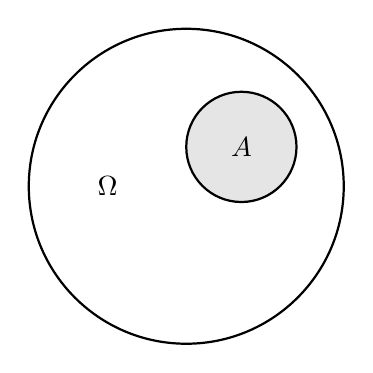
\begin{tikzpicture}[scale=1]
        \draw[thick] (0,0) circle (2cm);
        \node at (-1,0) {$\Omega$};
        \draw[thick, fill=gray!20] (0.7,0.5) circle (0.7cm);
        \node at (0.7,0.5) {$A$};
    \end{tikzpicture}
    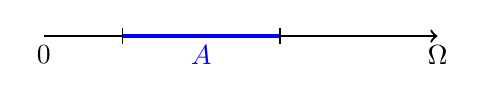
\begin{tikzpicture}[scale=1]
        \draw[thick,->] (0,0) -- (5,0);
        \node[below] at (0,0) {0};
        \node[below] at (5,0) {$\Omega$};
        \draw[very thick,blue] (1,0) -- (3,0);
        \node[below,blue] at (2,0) {$A$};
        \draw (1,0.1) -- (1,-0.1);
        \draw (3,0.1) -- (3,-0.1);
    \end{tikzpicture}
    \caption{Continuous random variables}
\end{figure}
Formally, if each event in A is equally likely, then
\begin{equation}
    P[\{x \in A\}] = \frac{\int_{A}dx}{|\Omega|}
\end{equation}
If we relax the assumption of equiprobability, then
more generally
\begin{equation}
    P[\{x\in A\}] = \int_{A} f_X(x) dx
\end{equation}
$f_X(x)$ is called the \emph{probability density function} (PDF).
It is analogous to the probability mass function.

Formally, a probability density function
is a mapping $f_X: \Omega \implies \Re$,
with the following properties:
\begin{itemize}
    \item Non-negativity: $f_X(x) \geq 0 \forall x \in \Omega$
    \item Unity: $\int_{\Omega} f_X(x)dx = 1$
    \item Measure of a set: $P[\{x \in A\}] = \int_{A}f_X(x) dx$
\end{itemize}

We can express a PDF in terms of a PMF
with a train of delta functions like so:
\begin{equation}
    f_X(x) = \sum_{x_k \in \Omega} p_X(x_k) \delta(x - x_k)
\end{equation}

We can also define the probability density
function as the derivative of the CDF, like so:
\begin{equation}
    f_X(x) = \frac{d}{dx}p(X \leq x)
\end{equation}

The expectation of a continuous random variable is
\begin{equation}
    E[X] = \int_{\Omega} xf_X(x)dx
\end{equation}

Properties of the expectation for continuous
random variables:
\begin{itemize}
    \item $E[aX] = aE[X]$
    \item $E[X+a] = E[X] + a$
    \item $E[aX+b] = aE[X] + b$
\end{itemize}

A random variable $X$ has an expectation
if it is absolutely integrable,
\begin{equation}
    E[|X|] = \int_{\Omega} |x|f_X(x)dx < \infty
\end{equation}

The variance of a continuous random variable
$X$ is
\begin{align}
    Var[X] & = E[(X-\mu)^2]                    \\
           & = \int_{\Omega} (x-\mu)^2f_X(x)dx \\
           & = E[X^2] - \mu^2
\end{align}